\documentclass[11pt,fleqn]{article}

\usepackage{blindtext}
\usepackage{hyperref}
\usepackage{fancyvrb}
\usepackage{graphicx}

\graphicspath{ {./} }

\hypersetup{
    colorlinks=true,
    linkcolor=blue,
    filecolor=magenta,      
    urlcolor=cyan,
    pdftitle={Design},
    pdfpagemode=FullScreen,
    }
\urlstyle{same}

\newcommand{\indentpar}{\phantom{=}}
\newcommand{\bli}{\begin{itemize}}
\newcommand{\eli}{\end{itemize}}

\begin{document}

    %% Title Page %%%%%%%%%%%%%%%%%%%%%%%%%%%%%%%%%%%%%%%%%%%%%%%%%
      
      \title{Design of VDisp Software}
      \date{\today}
      \author{Emil Soleymani, Dr.~Spencer Smith\\ McMaster University}
      \maketitle

      \medskip

      % Description
      \indentpar The \textbf{VDisp} software was carefully designed to adhere to the \href{https://www.digitalocean.com/community/conceptual_articles/s-o-l-i-d-the-first-five-principles-of-object-oriented-design}{\emph{SOLID} software design principles}.
      This document aims to outline the \hyperref[initialDesign]{initial proposed design} (which will be called the ideal design), the \hyperref[actualDesign]{actual implemented
      design}, and the \hyperref[juliaLimits]{limitations of the Julia programming language} that lead to this drastic change.
      
    %%%%%%%%%%%%%%%%%%%%%%%%%%%%%%%%%%%%%%%%%%%%%%%%%%%%%%%%%%%%%%%
    
    \pagebreak

    %% Ideal Design %%%%%%%%%%%%%%%%%%%%%%%%%%%%%%%%%%%%%%%%%%%%%%%
    \section*{Ideal Design} \label{initialDesign}

    \indentpar This section aims to describe the \emph{ideal} design which was drafted
    for the \textbf{VDisp} software. \\

    \begin{figure}[h]
        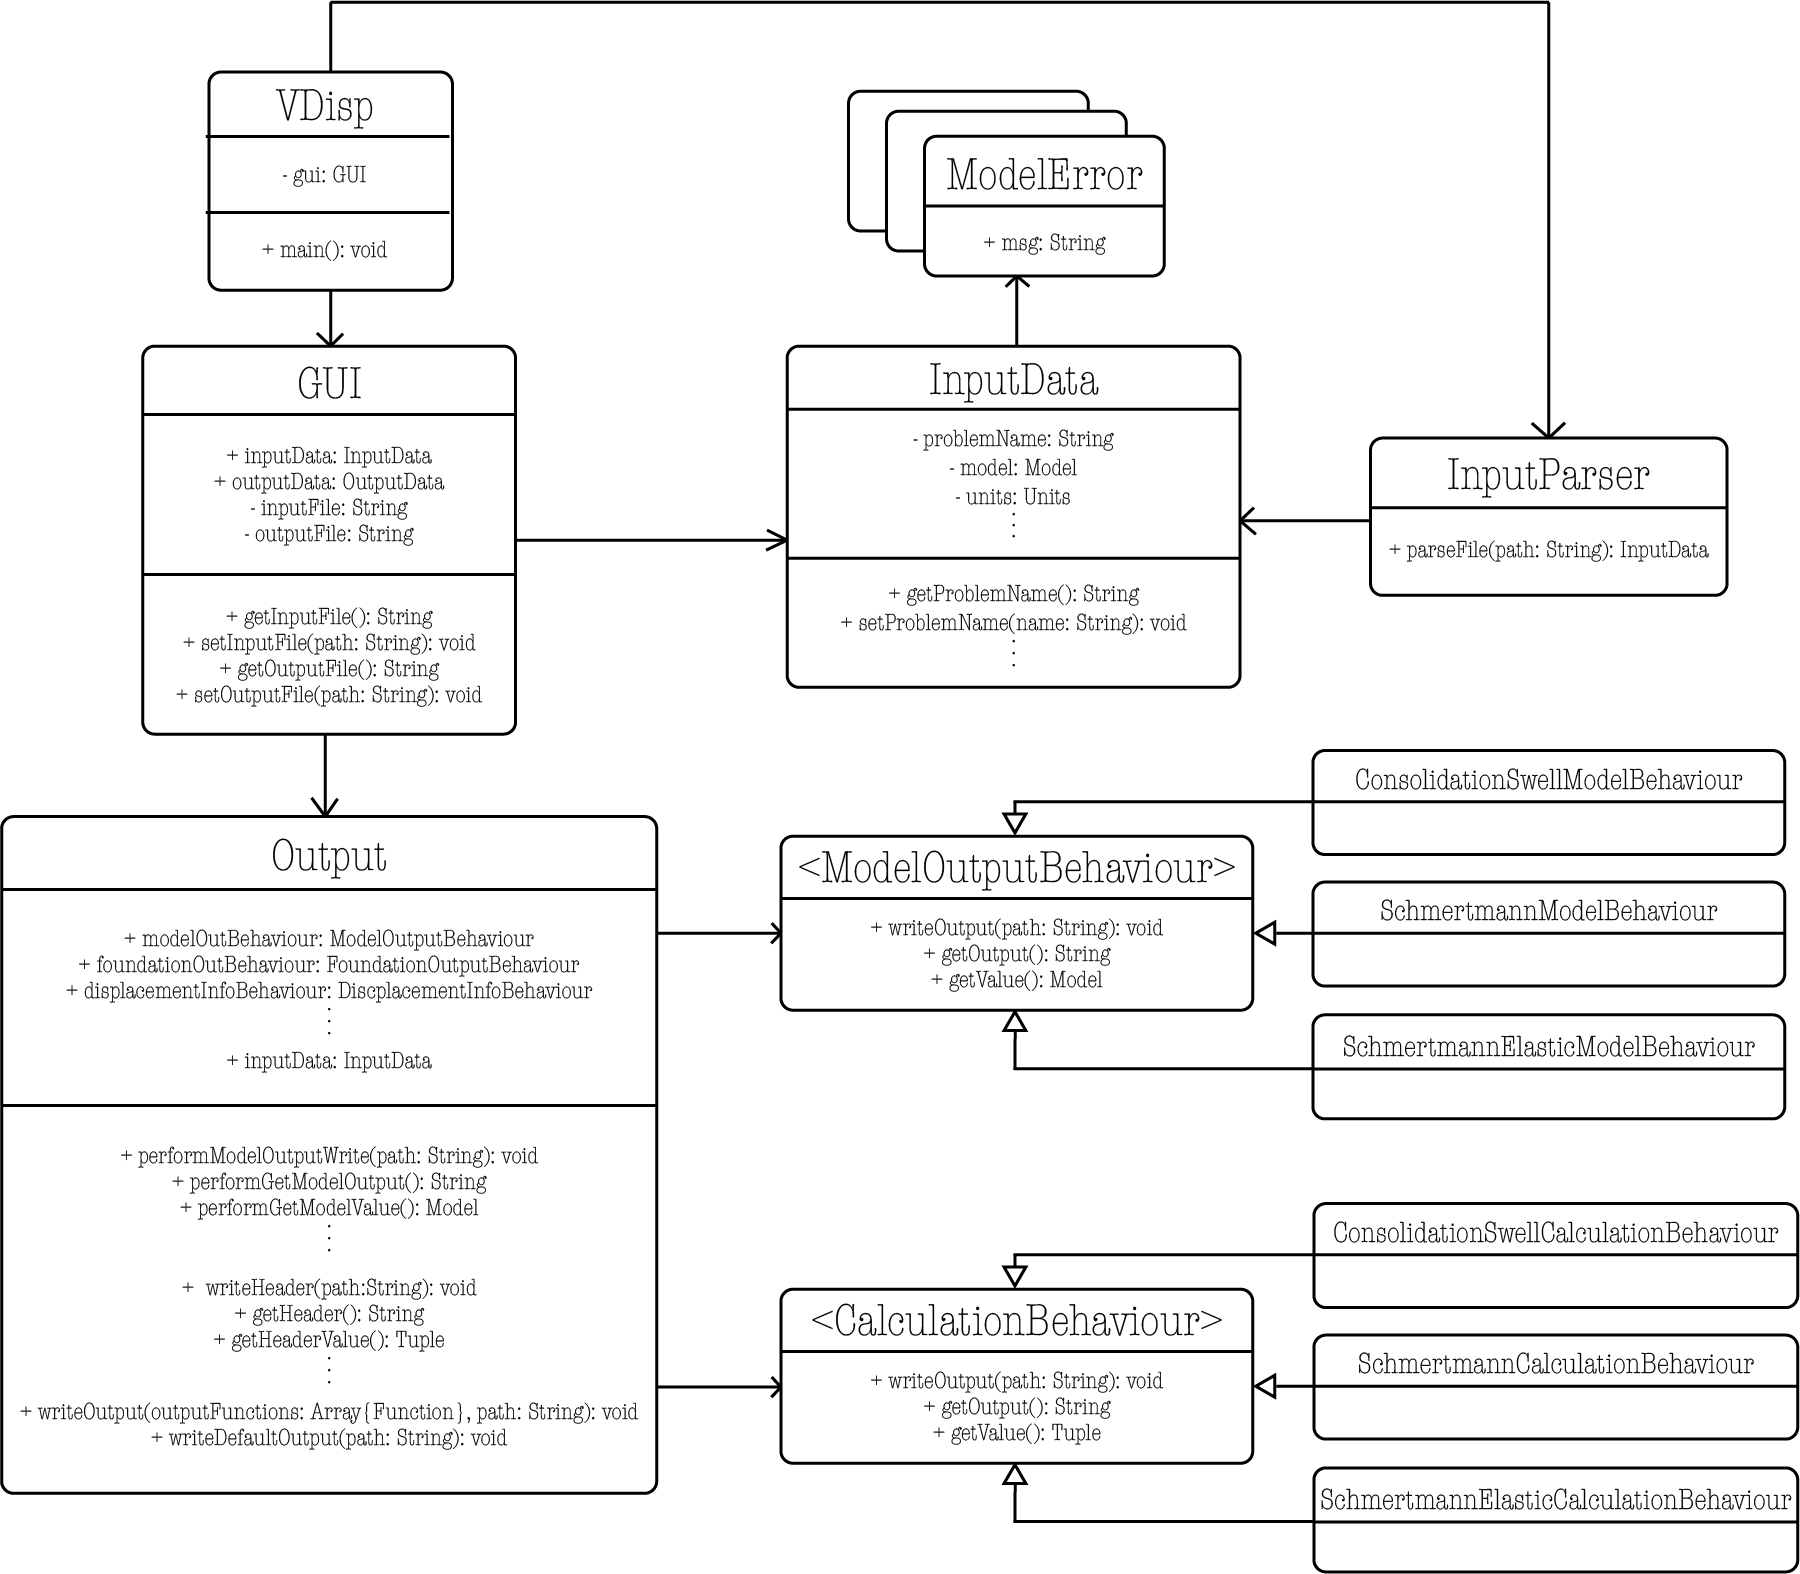
\includegraphics[width=1.3\textwidth]{VDispIdealDesignUML.png}
        \centering
    \end{figure}

    \indentpar The diagram above has been condensed. \emph{InputData} uses many 
    Custom Exception classes which help identify specific problems in the input file
    format allowing for helpful and descriptive messages to be given to the user. Furthermore,
    the \textbf{FoundationOutputBehaviour}, \textbf{DisplacementInfoBehaviour}, \textbf{ForcePointBehaviour} and
    \textbf{EquilibriumInfoBehaviour} interfaces (and the classes that implement them) have 
    been left out of the diagram. 
    
    \indentpar Examining the \textbf{ModelOutputBehaviour} interface is sufficient
    to understand the implementation of the excluded interfaces, while the \textbf{CalculationOutputBehaviour}
    is more complex than the other interfaces. The classes that implement \textbf{CalculationOutputBehaviour}
    are responsible for making method specific calculations, and return a set of values that is dependant on 
    the method itself. This is why the \textbf{CalculationOutputBehaviour} \emph{getValue()} function is said to
    return a \textbf{Tuple}. This \textbf{Tuple} contains different info based on the specified model, and classes
    that access this \textbf{Tuple} must be prepared to parse it.

    \indentpar The design pattern of the \emph{Output} class and the interfaces it uses (all the interfaces that 
    end in "\emph{Behaviour}") is inspired by the \emph{Duck example} in the opening chapter of \href{https://github.com/ksatria/MK-Design-Pattern/blob/master/Ebook/Head%20First%20Design%20Patterns.pdf}{this textbook}
    on design patterns.
    %%%%%%%%%%%%%%%%%%%%%%%%%%%%%%%%%%%%%%%%%%%%%%%%%%%%%%%%%%%%%%%
    
    %% Ideal Design %%%%%%%%%%%%%%%%%%%%%%%%%%%%%%%%%%%%%%%%%%%%%%%
    \section*{Actual Design} \label{actualDesign}

    \indentpar This section aims to describe the actual design which was implemented
    in the \textbf{VDisp} software. It strays from the \hyperref[initialDesign]{ideal design} due
    to some limitations outlined in the \hyperref[juliaLimits]{Julia Limitations} section.\\

    \indentpar At the moment, \emph{VDisp} is still being refactored, so the development 
    of an actual design UML diagram is being delayed.
    %%%%%%%%%%%%%%%%%%%%%%%%%%%%%%%%%%%%%%%%%%%%%%%%%%%%%%%%%%%%%%%
    
    %% Julia Limitations %%%%%%%%%%%%%%%%%%%%%%%%%%%%%%%%%%%%%%%%%%
    \section*{Julia Limitations} \label{juliaLimits}

    \indentpar This section aims to describe the limitations imposed
    upon us by Julia during development of the \emph{VDisp} software.
    These limitations mainly arose from the limited object-oriented capabilities
    of Julia — mainly importing structs from other modules.

    \subsection*{Importing Structs and Enums Between Modules}

        %%%%%%%%%%%%%%%%%%%%%%%%%%%%%%%%%%%%%%%%%%%%%%%%%%%%%%%%%%%%%%%

        \indentpar Suppose you wanted to define a struct that will hold all the 
        data the user inputs into the program. This is exactly what the \emph{InputData}
        struct aims to do. It is found in the \emph{InputParser.jl} module. Suppose 
        there is a function within \emph{InputParser.jl} that takes an argument which
        must be an instance of \emph{InputData}:
        
        \begin{verbatim}
        function doSomething(inputData::InputData)
            # Do stuff
        end
        \end{verbatim}

        \indentpar Now suppose you would like to use this function in another module,
        \emph{MyModule.jl}. You would first have to import the \emph{InputParser.jl}
        module, then create an instance of \emph{InputData}. Then you can try calling
        the function, and would feel confident that the following code produces no errors:

        \begin{verbatim}
        using InputParser

        inputData = InputData(...args)
        doSomething(inputData)
        \end{verbatim}

        \indentpar However, you get an error that says something along the lines of:

        \begin{verbatim}
        MethodError: 
        No function found for doSomething(
            Main.MyModule.InputParser.InputData)

        Closest Methods:
        doSomething(Main.InputParser.InputData)
        \end{verbatim}

        \indentpar I'm guessing this happens because Julia “copies” over the \emph{InputParser.jl}
        module into the \emph{MyModule.jl} file at compilation time due to the \emph{using InputParser}
        statement.

        \indentpar This behavior also caused many problems in the \emph{VDisp} custom exceptions which 
        are defined to catch various different errors in the input files. These custom exceptions are
        defined as structs, and a sample declaration is given as follows:
        
        \begin{verbatim}
        struct MyException <: Exception
            field1::Type
            field2::Type
            MyException(a::Type, b::Type) = new(a, b) 
        end
        \end{verbatim}

        Suppose this struct is defined in the \emph{InputParser.jl} module. Now suppose there is a function, \emph{parse(file)}, 
        in the same module that parses input files, and potentially throws \emph{MyException} or other exceptions.
        If we call this function from another module, maybe \emph{MyModule.jl}, we would again have to first import 
        the \emph{InputParser.jl} module, then call the \emph{parse(file)} function. Since this function can throw errors,
        we will catch them to be safe. Say we wanted to print \emph{foo} if a \emph{MyException} was thrown, else print \emph{bar}.
        One would expect the following code to get the job done:

        \begin{verbatim}
        using InputParser
        
        try
            parse("file.dat")
        catch e
            if isa(e, MyException)
                println("foo")
            else
                println("bar")
            end
        end
        \end{verbatim}

        \indentpar However, even if \emph{parse(“file.dat“)} does indeed throw a \emph{MyException},
        the code snippet above will still output \emph{bar}. To further investigate what is going on 
        here, try the following code:

        \begin{verbatim}
        using InputParser
        
        try
            parse("file.dat")
        catch e
            println(typeof(e))
        end
        \end{verbatim}

        \indentpar This code produces the output \emph{Main.MyModule.InputParser.MyException}. Thus, the original
        if statement condition, \emph{isa(e, MyException)}, was not true since \emph{Main.MyModule.InputParser.MyException}
        $\not =$ \emph{Main.InputParser.MyException}.

        \indentpar \emph{VDisp} does implement custom functions, so clearly there was a workaround. However,
        this was more of a “hack” — not a permanent, sustainable, scalable fix. There is an Enum called \emph{ErrorId}
        defined in the \emph{InputParser.jl} class (implemented using the \emph{@enum} macro). Each custom defined 
        exception has a corresponding \emph{ErrorId}, which is stored in each struct's \emph{id} field. Thus, the following
        code will achieve what we want:

        \begin{verbatim}
        using InputParser
        
        try
            parse("file.dat")
        catch e
            if Int(e.id) == Int(MyExceptionId)
                println("foo")
            else
                println("bar")
            end
        end
        \end{verbatim}

        \indentpar This code is assuming \emph{MyExceptionId} is properly defined in the \emph{InputParser.jl}
        module (\emph{@enum ErrorId MyExceptionId ...}), and that the \emph{id} of every \emph{MyException} is 
        set to \emph{MyExceptionId}. More careful readers may be wondering why the conditional was stated as 
        \emph{Int(e.id) == Int(MyExceptionId)}. Directly checking \emph{isa(e.id, MyExceptionId)} results in the
        same issue that we began with. However, we can convert any instance of an enum to its corresponding integer 
        value by wrapping it in the \emph{Int()} function. Now we can catch specific runtime errors, and perform the 
        necessary operations. Although omitted from the above code, it would be best practice to first check if 
        the error \emph{e} has a field called \emph{id} in the first place. This would arise if you accidentally forgot 
        to give a new error an \emph{id} field, or an exception was raised that is not one of your custom defined exceptions.   
        
        %%%%%%%%%%%%%%%%%%%%%%%%%%%%%%%%%%%%%%%%%%%%%%%%%%%%%%%%%%%%%%%

    \subsection*{QML.jl Package}
        %%%%%%%%%%%%%%%%%%%%%%%%%%%%%%%%%%%%%%%%%%%%%%%%%%%%%%%%%%%%%%%
        \indentpar Although the Julia community has grown significantly
        over the years, the options for 3rd party packages are still limited
        compared to that of more mature and ubiquitous languages like Python.
        This was especially problematic when it was time to choose a library 
        to draw the graphics for the user interface. The best option was the 
        \emph{QML.jl} package, which used another package, \emph{CxxWrap.jl},
        to communicate desired Qt/QML functionality to its native language, C++.
        This package is developed and maintained by a single person, so naturally
        it cannot be as robust and complete as a package like \emph{Tkinter} or 
        \emph{pygame}.

        \indentpar The biggest problem related to the \emph{QML.jl} package came up
        when \emph{VDisp} needed to execute a function contained in its Julia code on 
        a certain UI event triggered in the QML markup. For example, if we wanted to run 
        Julia code in a function called \emph{saveFile()} when clicking on a button defined
        in a QML file, we would have to first “pass the function“ into QML by calling the 
        \emph{@qmlfunction saveFile} macro, then have a QML file as follows:

        \begin{verbatim}
            import import QtQuick 2.12
            import org.julialang 1.0

            Rectangle{
                /* Design */
                
                MouseArea {
                    anchors.fill: parent
                    onClicked: Julia.saveFile  // Call saveFile()
                }
            }
        \end{verbatim}
        
        \indentpar Although this is the method found in the \emph{QML.jl} documentation,
        and it was used in a demo UI created to test the package before choosing it
        for this project (see \href{https://github.com/EmilSoleymani/JuliaThermostat}{this} 
        GitHub repo), when trying to call functions from the UI the following error 
        occurred:
        
        \begin{center}
        \begin{BVerbatim}
        ERROR: LoadError: Could not find module QML when looking up function 
        get_julia_call
        
        Stacktrace:
        [1] exec()
        @ QML ~/.julia/packages/CxxWrap/ptbgM/src/CxxWrap.jl:619
        \end{BVerbatim}
        \end{center}

        \indentpar There seems to be a bug within the \emph{CxxWrap.jl} library,
        or in the use of this library within the \emph{QML.jl} package. 

        \indentpar Once again, \emph{VDisp} uses a “hack” to get around this. This is 
        by no means a scalable, permanent solution to the problem, but it serves as a 
        way to get the application working until the developers update the packages. 
        \emph{QML.jl} allows developers to pass in \emph{Observable} variables (from 
        the \emph{Observables.jl} package) into the \emph{loadqml()} function which can 
        be accessed globally in the QML files. Any changes made to these variables through
        the UI logic described in the QML files will be relayed to the variables in Julia.
        The \emph{Observables.jl} package allows developers to define an “observer” function
        which executes each time an \emph{Observable} variable's value is changed (I'm guessing
        the name of the package comes from the Observer design pattern which is used in the 
        underlying code). Using this functionality, we can create an \emph{Observable} variable 
        with a boolean value, pass it into QML, set it to true when we want to execute a function,
        and call the function from the \emph{Observable}'s observer function. This will be easier
        for readers to digest after examining the refactored code of the example above which 
        implements this method:
        
        \begin{verbatim}
        using Observables

        # init Observable variable to be false by default
        executeSaveFile = Observable(false)
        
        # define observer function for executeSaveFile
        saveFileObserver = on(executeSaveFile) do val
            # if the new value of executeSaveFile is true
            if val
                saveFile()  # call function
            end
        end

        # Load qml file and pass in executeSaveFile as variable
        loadqml("main.qml", executeSaveFile=executeSaveFile)
        \end{verbatim}

        \indentpar Now, the QML file will be refactored to:

        \begin{verbatim}
            import import QtQuick 2.12
            import org.julialang 1.0

            Rectangle{
                /* Design */
                
                MouseArea {
                    anchors.fill: parent
                    onClicked: executeSaveFile = true  // Call saveFile()
                }
            }
        \end{verbatim}
        %%%%%%%%%%%%%%%%%%%%%%%%%%%%%%%%%%%%%%%%%%%%%%%%%%%%%%%%%%%%%%%

    %%%%%%%%%%%%%%%%%%%%%%%%%%%%%%%%%%%%%%%%%%%%%%%%%%%%%%%%%%%%%%%

\end{document}